% !TeX encoding = UTF-8
% !TeX spellcheck = de_DE

%% Dies gibt Warnungen aus, sollten veraltete LaTeX-Befehle verwendet werden
\RequirePackage[l2tabu, orthodox]{nag}

\documentclass[utf8,biblatex]{lni}
\bibliography{bibliographie}

%% Schöne Tabellen mittels \toprule, \midrule, \bottomrule
\usepackage{booktabs}

%% Zu Demonstrationszwecken
\usepackage[math]{blindtext}
\usepackage{mwe}

%% BibLaTeX-Sonderkonfiguration,
%% falls man schnell eine existierende Bibliographie wiederverwenden will, aber nicht die .bib-Datei händisch anpassen möchte.
%% Bitte \iffalse und \fi entfernen, dann ist diese Konfiguration aktiviert.

\iffalse
\AtEveryBibitem{%
  \ifentrytype{article}{%
  }{%
    \clearfield{doi}%
    \clearfield{issn}%
    \clearfield{url}%
    \clearfield{urldate}%
  }%
  \ifentrytype{inproceedings}{%
  }{%
    \clearfield{doi}%
    \clearfield{issn}%
    \clearfield{url}%
    \clearfield{urldate}%
  }%
}
\fi

\begin{document}
%%% Mehrere Autoren werden durch \and voneinander getrennt.
%%% Die Fußnote enthält die Adresse sowie eine E-Mail-Adresse.
%%% Das optionale Argument (sofern angegeben) wird für die Kopfzeile verwendet.
\title[Green IT]{Green IT - Wie kann der Verbrauch natürlicher Ressourcen in der IT-Branche reduziert werden?}
%%%\subtitle{Untertitel / Subtitle} % if needed
\author[Fabian Heinl \and Philipp Kremling]
{Fabian Heinl\footnote{Duale Hochschule Baden Württemberg, Campus Horb, Florianstraße 15, 72160 Horb,
Deutschland \email{i20014@hb.dhbw-stuttgart.de}} \and
Philipp Kremling\footnote{Duale Hochschule Baden Württemberg, Campus Horb, Florianstraße 15, 72160 Horb,
Deutschland \email{i20022@hb.dhbw-stuttgart.de}}}
\startpage{1} % Beginn der Seitenzählung für diesen Beitrag / Start page
\editor{DHBW Stuttgart, Campus Horb} % Names of Editors
\booktitle{Advanced Software Engineering} % Name of book title
\yearofpublication{2022}
%%%\lnidoi{18.18420/provided-by-editor-02} % Falls bekannt


\maketitle

\begin{abstract}
Gerade heutzutage, inmitten des menschengemachten Klimawandels und mit immer weiter steigenden Energiepreisen, die eine Belastung für Unternehmen und Privathaushalte darstellen, ist es wichtig natürliche Ressourcen zu schonen und Strom zu sparen. Speziell die IT-Branche verbraucht durch Rechenzentren und immer mehr Software viel Energie. Der Ansatz Green IT beschreibt Herangehensweisen, wie der natürliche Ressourcenverbrauch von Software reduziert werden kann. In dieser Arbeit wird zunächst betrachtet, wie der natürliche Ressourcenverbrauch von Software messbar ist. Auch die aktuell eher gegensätzliche Bewegung im Bereich des Cloud Computings wird beschrieben. Anschließend werden konkrete Umsetzungsmöglichkeiten beschrieben werden. Hierbei liegt der Fokus auf der verwendeten Software-Architektur, Software-Pattern und Vorgehensmodellen. Zudem ist es wichtig, zu gewährleisten, dass die Software auch zukünftig nachhaltig bleibt, wozu im Anschluss Möglichkeiten evaluiert werden. Abschließend erfolgt eine Bewertung der vorgestellten Umsetzungsmöglichkeiten, die sowohl wirtschaftliche Aspekte und die Ressourceneinsparung, aber auch die Schwächen des Ansatzes herausstellt.
\end{abstract}

\begin{keywords}
Software Engineering \and Green IT \and Green Software Engineering
\end{keywords}

\section{Einleitung}
Im folgenden Kapitel soll der Leser oder die Leserin mit der Arbeit vertraut gemacht werden: Es wird dafür zunächst die Motivation und der generelle Aufbau der Arbeit erläutert. 
\newline
Im Zuge der besseren Lesbarkeit wird im Folgenden ausschließlich das generische Maskulinum verwendet. Alle weiteren Geschlechter sind hier jedoch gleichermaßen mit eingeschlossen.

\subsection{Motivation}
Die Erde wärmt sich durch den menschengemachten Klimawandel immer weiter auf. So war die durchschnittliche Temperatur 2021 um 1,11° höher im Vergleich zum vor-industriellen Level. \cite{WMO22} Dies hat dramatische Auswirkungen auf unseren Planeten und zeigt sich in immer stärkeren und heftigeren Naturkatastrophen. Als Beispiele seien hier die Dürre in Europa oder das Jahrhunderthochwasser in Australien im Jahr 2022 genannt. Ein Hauptgrund der Erwärmung ist dabei der anthropogene Treibhauseffekt \cite{bpb22}. Dabei ist der Energiesektor in Deutschland mit 82,8\% die größte Quelle für Treibhausgase im Jahr 2020. \cite{UBA22} 
\newline \newline
Speziell die IT-Branche verbraucht durch Rechenzentren und immer mehr Software viel Energie. War der Informations- und Kommunikationssektor 2007 noch für 1,5\% des weltweiten CO2-Fußabdrucks verantwortlich, so wird vermutet, dass es 2040 bereits 14\% sein werden. \cite{Podder20} Vor allem der Energiebedarf von Servern in deutschen Rechenzentren wird laut Facheinschätzungen von 2015 bis 2025 um mehr als 60\% steigen. \cite{BMUV20} Aus diesem Grund werden vermehrt auch hier Strategien gefordert, mittels derer die IT-Branche ressourcenschonender auftreten kann. Zudem bei immer weiter steigenden Energiepreisen, die eine Belastung für Unternehmen und auch Privathaushalte darstellen, eine energieschonendere Soft- und Hardware auch wirtschaftliche Vorteile bietet. So besteht nicht nur beim Stromverbrauch Potenzial zum Einsparen, sondern auch bei der Herstellung und dem Recycling von Computern und deren Komponenten.\cite{Murugesan08}
\newline \newline
Der Ansatz Green IT beschreibt dabei Herangehensweisen, wie der natürliche Ressourcenverbrauch von Software reduziert werden kann. Hierbei muss der gesamte Lebenszyklus des Software-Produkts betrachtet werden. So muss während der Entwicklung ein ressourcenschonender Umgang der Technik im Betrieb, aber auch die umweltschonende Entsorgung und Wiederverwendung der Einsatzmaterialien Berücksichtigung finden. \cite{Lackes18}
\newline \newline
Die Vorteile von Green IT liegen auf der Hand: Indem der Ressourcenverbrauch von Software reduziert wird, verbraucht das Unternehmen weniger Strom und spart somit Geld. Auch nach außen hin wird durch einen geringeren Stromverbrauch die indirekte Produktion von CO2 durch die Stromherstellung reduziert. So können auch IT-Unternehmen einen aktiven und nicht zu unterschätzenden Beitrag zur Verringerung des Klimawandels leisten.
\newline \newline
In dieser Arbeit wird zunächst betrachtet, wie der natürliche Ressourcenverbrauch von Software messbar ist. Anschließend werden konkrete Umsetzungsmöglichkeiten beschrieben. Diese Umsetzungsmöglichkeiten reichen von der verwendeten Hardware bis zur Softwarearchitektur und Software-Pattern. Zudem ist es wichtig, zu gewährleisten, dass die Software auch zukünftig nachhaltig bleibt. Abschließend erfolgt eine Bewertung der vorgestellten Umsetzungsmöglichkeiten, die sowohl wirtschaftliche Aspekte und die Ressourceneinsparung, aber auch die Schwächen des Ansatzes herausstellen soll.

\subsection{Aufbau der Arbeit}
Der Aufbau der Arbeit soll den Gedankengängen des Lesers folgen. Begonnen wird deshalb mit Green IT generell. Zunächst wird dieses Konzept definiert. Dabei soll vor allem die Sinnhaftigkeit des Konzepts verdeutlicht werden.\newline
Anschließend wird erläutert, wie der natürliche Ressourcenverbrauch von Software messbar ist und es werden aktuelle Entwicklungen im Bereich Green IT aufgezeigt, so zum Beispiel im Bereich des Cloud Computings. Dabei wird insbesondere darauf eingegangen, dass aktuell eher entgegengerichtete Ansätze zu Green IT sichtbar sind. 
\newline
\newline
Nachdem die Grundlagen zu Green IT erläutert wurden, sollen konkrete Umsetzungsmöglichkeiten erklärt werden. Hierbei wird zunächst auf die Softwarearchitektur eingegangen. Auch diese hat einen Einfluss darauf, wie viele natürliche Ressourcen eine Software verbraucht. Es sollen dabei verschiedene Architekturtypen gegenübergestellt werden.
\newline
Anschließend werden bestimmte Software-Patterns beachtet durch die eine effizientere Software geschaffen und so der natürliche Ressourcenverbrauch durch diese reduziert werden kann. 
\newline
Abschließend wird auch der Einfluss von Vorgehensmodellen während der Entwicklung eines Software-Produkts betrachtet. Auch diese können einen Einfluss auf den natürlichen Ressourcenverbrauch einer Software haben. Speziell agile Vorgehensweisen können mit Blick auf diese Tatsache optimiert werden.
\newline
\newline
Bisher wurde lediglich betrachtet, wie eine Software anfangs so erstellt werden kann, dass sie möglichst ressourcenschonend ist. Wenn diese Eigenschaft jedoch im weiteren Lebenszyklus des Software-Produkts vernachlässigt wird, ist dies nicht ausreichend. Aus diesem Grund wird anschließend auf Möglichkeiten eingegangen, wie gewährleistet werden kann, dass die Software auch zukünftig nachhaltig bleibt.
\newline
\newline
Im Anschluss werden das generelle Konzept Green IT und die verschiedenen vorgestellten Umsetzungsmöglichkeiten bewertet. Hierbei werden Aspekte der CO2- und Ressourceneinsparung, aber auch wirtschaftliche Aspekte und Schwächen des Ansatzes wie Greenwashing, wirtschaftliche Widersprüchlichkeit und Reboundeffekte betrachtet.
\newline
Abschließend soll ein Ausblick gegeben werden, der nochmals die Vorteile von Green IT aufzeigt und weitere mögliche Verbesserungen und Entwicklungen in der Zukunft beschreibt.

\section{Green IT}
\label{GreenIT}
Green IT ist ein Begriff der auch durch die steigende Bedrohung durch den Klimawandel immer mehr Entwicklern bekannt wird. Dieser Begriff bezieht sich nicht nur auf den enormen Stromverbrauch durch Software oder durch die allgemeine IT-Infrastruktur, was auch der Öffentlichkeit in letzter Zeit bewusster wird. So wurde neben dem Energieverbrauch des Internets im Zuge des Bitcoin-Hypes auch viel über den enormen Stromverbrauch, der für das Minen der Kryptowährung nötig ist, in den Medien berichtet. Im Jahr 2020 wurden allein beim Mining für Bitcoins 75,4 TWh verbraucht, was mehr als der Bedarf Österreichs mit 69,9 TWh entspricht. \cite{ZDF22}. Nicht nur in Bezug auf Bitcoins und das Internet wäre es also von Vorteil, wenn beim Betrieb von Software Energie gespart werden könnte. So gehen Experten davon aus, dass die Nachfrage an Rechenleistung allein in deutschen Rechenzentren von 2015 bis 2025 um mehr als 60\% steigt. \cite{BMUV20}

Green IT bezieht sich jedoch nicht nur auf den Stromverbrauch, auch wenn dieser das Hauptaugenmerk dieser Arbeit ist. So wird im Gabler Wirtschaftslexikon folgende Definition gegeben: „[Green IT] bezeichnet die ressourcenschonende Verwendung von Energie und Einsatzmaterialen in der Informations- und Kommunikationstechnologie über den gesamten Lebenszyklus hinweg, d. h. dass bereits bei der Entwicklung nicht nur ein möglichst ressourcenschonender Umgang der Technik im Betrieb, sondern auch eine umweltschonende Entsorgung und Wiederverwendung der Einsatzmaterialien Berücksichtigung findet.“ \cite{Lackes18} Es wird also nicht nur der Betrieb, wie z. B. der Ressourcenverbrauch von Rechenzentren, beachtet und versucht klimafreundlicher zu gestalten. Auch bei der Entwicklung der Anwendungen und dem Aufbau von Infrastrukturen soll auf Ressourcenschonung geachtet werden. Hierzu werden im Folgenden einige Beispiele gegeben. Auch der Umgang mit der Hardware muss als weiterer Aspekt neben der Software Beachtung finden. Diese soll nicht nur möglichst klimafreundlich produziert und z. B. durch Ökostrom betrieben werden, auch bei der Entsorgung muss auf umweltschonende Prozesse und Recycling geachtet werden.

Im Rahmen dieser Arbeit wird der Fokus jedoch auf die Ansätze für ressourcenschonendere Softwareentwicklung (auch als Green Software Engineering bekannt) gelegt. So wird zwar durch Hardware die Energie verbraucht, jedoch wird der Energieverbrauch von der Software erst ausgelöst. Asmin Hussain, Leiter der Interessensvertretung für Green Cloud Computing bei Microsoft, beschreibt zwei Philosophien grüner Softwareerstellung: Zum einen hat jeder einen Teil an der Lösung des Klimawandels und somit einen Einfluss auf die Zukunft. Zum anderen gibt es viele Vorteile bei nachhaltiger Software: Diese sind oft günstiger, performanter und resilienter. Der Aspekt der Nachhaltigkeit sollte jedoch der Hauptfokus von Green Software Engineering sein. Liegt der Fokus stattdessen z. B. auf Performanz, kann der Aspekt der Nachhaltigkeit schnell vernachlässigt werden. Neben den Philosophien können laut Hussain unabhängig von Anwendungsbereich, Industriebereich, Größe oder Art der Organisation, Hosting und Programmiersprache acht Prinzipien der nachhaltigen Softwareentwicklung Beachtung finden: „Carbon, Electricity, Carbon Intensity, Embodied Carbon, Energy Proportionality, Networking, Demand Shaping [und] Measurement \& Optimization“ \cite{Principles21} Diese zielen nicht alle direkt auf den Stromverbrauch ab, sind jedoch für das Ziel ressourcenschonender IT auch ein wichtiger Faktor, weshalb diese Folgend ein weniger genauer beleuchtet werden.

\textit{Carbon} \newline
Treibhausgase sind durch ihre wärmende Wirkung ein Faktor, warum Leben auf der Erde überhaupt möglich ist. Durch den Ausstoß großer Mengen von Treibhausgasen, den die Menschheit seit der industriellen Revolution verursacht, ändert sich jedoch das Klima schneller, als sich Flora und Fauna anpassen können. Das von den Vereinten Nationen aufgestellte und von 195 Staaten unterzeichnete Pariser Klimaabkommen, versucht dem entgegenzuwirken. Es zielt darauf ab den Kohlenstoffausstoß zu minimieren und so den Temperaturanstieg bis 2100 um 1,5°C im Vergleich zu vorindustriellen Werten zu stabilisieren. Anwendungen sollen also für jedes Gramm Kohlenstoff, das ausgestoßen wird, den gleichen Mehrwert für Nutzer bieten, aber weniger CO2-Emmisionen verursachen.

\textit{Electricity} \newline
Der meiste Strom wird durch die Verbrennung fossiler Brennstoffe erzeugt. Auch beim vorher erwähnten Beispiel Bitcoin-Mining ist dies der Fall. So werden in vielen Fällen Kohlekraftwerke zur Erzeugung des benötigten Stroms verwendet. Es kann also eine Beziehung zwischen Stromverbrauch von Software und Treibhausgasemission hergestellt werden. So beginnt es nicht beim Computer und den Anwendungen an sich, sondern schon bei der Herstellung des Stroms. Indem ein Entwickler den Energieverbrauch seiner Programme minimiert, wird ebenfalls Energie eingespart. Eine Möglichkeit dafür ist die Verwendung effizienterer Algorithmen, um so ein leistungsfähigeres Programm zu schaffen. \cite{Principles21}

\textit{Carbon Intensity} \newline
Die Kohlenstoffintensität beschreibt, wie viele Kohlenstoffemissionen pro verbrauchter Kilowattstunde Strom entstehen, also wie viel Kohlenstoff pro Kilowattstunde ausgestoßen wird. Ist ein Computer z. B. direkt an einem Wasserkraftwerk oder einer Solaranlage angeschlossen, wäre die Kohlenstoffintensität gleich null, vorausgesetzt diese nachhaltigen Methoden produzieren genug Strom. Die Kohlenstoffintensität ändert sich je nach Standort, da überall ein unterschiedlicher Energiemix vorhanden ist. Das Problem mit erneuerbaren Energien ist jedoch, dass diese nicht immer gleichmäßig vorhanden und von der Wetterlage abhängig sind. Als Basis werden deshalb im Stromnetz fossile Energien benutzt, um dem Gesamtverbrauch gerecht zu werden. Strom aus erneuerbaren Energien wird bei einem größeren Angebot als Nachfrage gekürzt. Ist man als Softwareentwickler flexibel in der Ausführung der Arbeitslasten, kann in einem solchen Fall die Nachfrage erhöht werden und so die geringere Kohlenstoffintensität ausnutzen. So ist es z. B. möglich, dass ein maschinelles Lernmodell in einer Region oder zu einem Zeitpunkt trainiert wird, zu dem viele erneuerbare Energien im Energiemix enthalten sind, sodass weniger Kohlenstoff ausgestoßen wird. Studien konnten zeigen, dass Maßnahmen solche Maßnahmen, je nach Anzahl der erneuerbaren Energien im Stromnetz, den ausgestoßenen Kohlenstoff um 45 – 99\% reduzieren Konten. \cite{Kelly11}

\textit{Embodied Carbon} \newline
Für die Herstellung jedes Geräts, darunter z. B. auch Komponenten für Server, wurde bei deren Herstellung Kohlenstoff freigesetzt. Auch am Ende der Lebensdauer des Geräts kann durch die Entsorgung Kohlenstoff freigesetzt werden. Bei der Berechnung der Kohlenstofffreisetzung einer Hardwarekomponente dürfen also nicht nur die Kosten für den Betrieb einberechnet werden, sondern auch die der Herstellung und Entsorgung. Vermindern kann man diesen Wert durch die Verlängerung der Nutzungsdauer von Hardware. So werden alte Geräte entfernt, weil diese defekt oder nicht mehr in der Lage sind, neue Aufgaben zu bewältigen. Defekte Geräte lassen sich aus Sicht des Softwareentwicklers nicht vermeiden. Wird Software jedoch so entwickelt, dass weniger Geräte überlastet werden, müssen diese nicht durch leistungsstärkere Geräte ersetzt werden. Zudem können Anwendungen auch so entwickelt werden, dass diese von älterer Hardware noch genutzt werden können.

\textit{Energy Proportionality} \newline
Die Auslastung gibt an, wie stark die Ressourcen eines Computers genutzt werden. Im Leerlauf ist diese geringer als bei voller Last. Die Energieproportionalität ist ein Maß für das Verhältnis von verbrauchter Energie und der Auslastung einer Hardware-Komponente. Im Fall von Hardwarekomponenten ist die Energieproportionalität nicht konstant und variiert je nach Kontext. So verbraucht ein Computer bei 0\% Auslastung z. B. 100W, bei 50\% 180W und bei 100\% 200W an Energie. Je mehr die Hardware genutzt wird, desto effizienter ist diese bei der Umwandlung von Strom in Rechenoperationen. Werden also möglichst wenig Server auf höchster Auslastung beschäftigt, maximiert man deren Energieeffizienz.

\textit{Networking} \newline
Das Internet besteht aus einer großen Menge von Routern und Servern und anderen Geräten. Diese verbrauchen Strom und setzen so abhängig von der lokalen Kohlenstoffintensität auch Kohlenstoff frei. So erzeugen alle Daten, die man über das Internet sendet oder empfängt, Kohlenstoffemissionen. Diese sind abhängig vom Umfang der Daten, Entfernung, Anzahl der Sprünge zwischen Netzwerkgeräten, Energieeffizienz dieser, der Kohlenstoffintensität der verwendeten Energie und dem Netzwerkprotokoll. Als wichtigste Faktoren gelten dabei die Größe und Entfernung der Pakete. Dieser Fakt kann bei der Konzipierung und Entwicklung der Software einbezogen werden, sodass z. B. die Größe der von einer Anwendung verschickten Pakete möglichst klein gehalten wird. \cite{Principles21}

\textit{Demand Shaping} \newline
Nachfragestrukturierung ist eine ähnliche Strategie wie die Nachfrageverschiebung. Statt die Rechenleistung örtlich oder zeitlich zu verlagern, wird hier die Energie-Nachfrage an das bestehende Angebot angepasst. Wenn also gerade viel erneuerbare Energie im Energiemix enthalten ist, wird auch der Umfang der Anwendung erhöht. So kann z. B. die Benutzererfahrung geändert werden, um die Kohlenstoffemissionen zu verringern. Dies ist vergleichbar mit Energiesparmodi, die z. B. in modernen Spül- und Waschmaschinen vorkommen. Sind diese eingeschaltet, wird die Leistung des Geräts gedrosselt, sodass für die Erfüllung derselben Aufgaben weniger Ressourcen verbraucht werden, indem z. B. die benötigte Zeit erhöht wird. Ob der Energiesparmodus eines Geräts durch Benutzer manuell eingestellt werden kann oder automatisch verwaltet wird, muss während der Entwicklung entschieden werden. Auf Kosten der Rechenleistung kann so also zusätzlich Kohlenstoff eingespart werden.

\textit{Measurement \& Optimization} \newline
Bei der Erstellung einer nachhaltigen Software, genügt nicht nur eine Optimierung, sondern es benötigt deutlich mehr. So muss die Anwendung im Ganzen betrachtet werden und von der Benutzererfahrung bis zur Vernetzung und den Rechenzentren schrittweise vorgegangen werden. Die Wahl der Messkriterien hat dabei einen großen Einfluss auf den Erfolg der Dekarbonisierung einer Anwendung. So ist es z. B. nicht sinnvoll bei einer Anwendung die Netzwerklast zu verringern, wenn die Datenbankabfragen deutlich häufiger vorkommen und deshalb deutlich mehr Kohlenstoff freisetzen. Die verbrauchte Energie einer Anwendung kann je nach Zeitpunkt und Ort variieren, jedoch ist weniger Stromverbrauch bei gleicher Leistung bereits ein guter Indikator, um die Nachhaltigkeit des Softwareprodukts zu bestimmen. Auch die Kosten für Strom und Hardware können als Indikator verwendet werden. So ist eine Anwendung, die keine hohe Last erzeugt, meist auch mit einem geringem Kohlenstoffausstoß verbunden. Auch die Vernetzung muss betrachtet werden. So kann durch Messung und anschließende Verringerung der Menge und Entfernung, die die Daten zurücklegen müssen, auch Kohlenstoff eingespart werden. \cite{Principles21} Die Messbarkeit von Green IT wird im nächsten Kapitel genauer erläutert.

\subsection{Messbarkeit}
Nachdem im letzten Kapitel der Grundbegriff Green IT näher betrachtet wurde, wird in diesem Kapitel auf die Messbarkeit der Einsparungen eingegangen. Die acht Prinzipien zeigen die verschiedenen Einsparpotenziale, die man bei nachhaltiger Softwareentwicklung beachten sollte.  Im Zuge dieser Arbeit wird dabei vor allem auf die Stromeinsprung eingegangen. Seit 2020 gibt es in Deutschland mit der Einführung des „Blauen Engels für ressourcen- und energieeffiziente Software“ ein für Endnutzer verlässliches Label, das eine grüne Software auszeichnet. \cite{Guldner22} Dabei werden die Anforderungen zum Erhalt des Labels in drei Bereiche eingeteilt: Ressourcen- und Energieeffizienz, potenzielle Hardware-Nutzungsdauer und Nutzungsautonomie. Ressourcen- und Energieeffizienz gibt dabei auch nützliche Anhaltspunkte zur Messbarkeit.

Als Bezugsgrößen zur Berechnung der Ressourcen- und Energieeffizienz werden die Hardwareressourcen und der Energieverbrauch verwendet. Mit Hilfe eines Referenzsystems wird die elektrische Leistungsaufnahme im Leerlauf gemessen. Dabei werden folgende Werte im Leerlauf ermittelt und der Mittelwert berechnet: Prozessorauslastung (\%), Arbeitsspeicherbelegung (Mbyte), Permanentspeicherbelegung (Mbyte/s), beanspruchte Bandbreite für Netzzugang (MBit/s) und die elektrische Leistungsaufnahme (W). Diese Daten sind über das Betriebssystem einsehbar und werden z. B. im Windows Task-Manager unter „Leistung“ visualisiert. Zusätzlich zur Leistung im Leerlauf wird für den Blauen Engel auch die Hardware-Inanspruchnahme und der Energiebedarf bei Ausführung eines Standardnutzungsszenarios beachtet. Grundlage ist dabei ein Referenzsystem, wobei nicht nur die zusätzliche Inanspruchnahme, sondern auch ein prozentualer Anteil der Grundauslastung bei der Berechnung einbezogen wird. Gemessen werden dabei Prozessorarbeit (\% * s), Arbeitsspeicherarbeit (Mbyte * s), Permanentspeicherarbeit (Lesen und Schreiben) (Mbyte/s * s), Übertragene Datenmenge für Netzzugang (MBit/s * s) und der Mittelwert des Energiebedarfs (Wh). Dabei ist darauf zu achten, dass die Software keinen Einfluss auf das Energiemanagement des Systems (z. B. Standby-Modus) hat und umgekehrt die Funktionalität der Software auch nicht durch etwaige Funktionen eingeschränkt wird. \cite{BlauerEngel20}

In \autoref{aufbau} wird ein beispielhafter Messaufbau erläutert, mit dem diese Messwerte ermittelt werden können. 
\begin{figure}[ht]
\centering
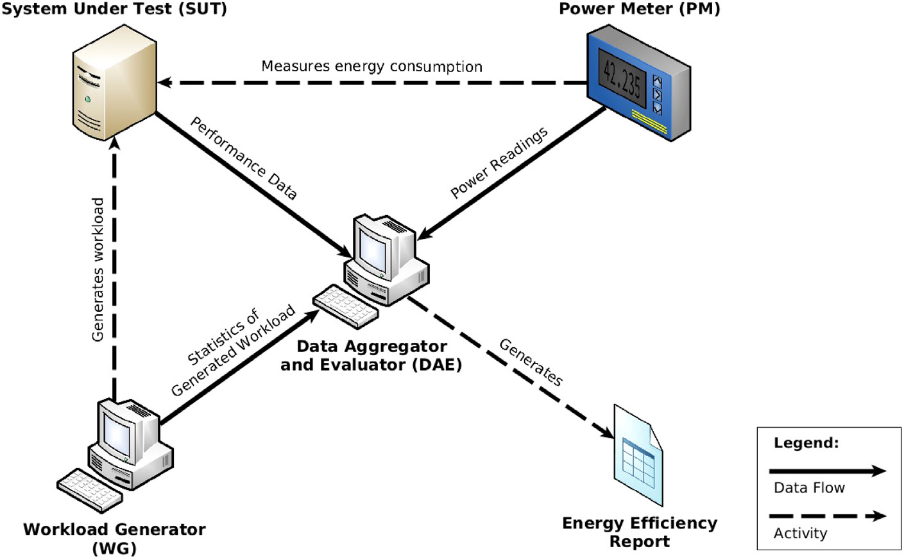
\includegraphics[width=0.9\linewidth]{Messbarkeit_Testaufbau.png}
\caption{{\centering 
Exemplarischer Aufbau zur Messung der Hardwareauslastung und des Energieverbrauchs eines Softwaresystems.\cite{Kern18}
}}
\label{aufbau}
\end{figure}
\newline
Wie in \autoref{aufbau} zu sehen, besteht der Testaufbau aus folgenden Komponenten: 
\begin{itemize}
\item System Under Test (SUT)
\item Leistungsmessgerät (PM)
\item Workload Generator (WG)
\item Datensammlung und -analyse (DAE)
\end{itemize}
Folgend werden die einzelnen Komponenten genauer erläutert und anschließend der Ablauf einer beispielhaften Messung erklärt:

\textit{System Under Test (SUT)} \newline
Bei einer Messung wird ein Szenario mit dem zu analysierenden Software-Produkt erstellt, welches dann auf dem SUT ausgeführt wird. Dabei besteht ein SUT z. B. aus einem PC, Server, Mobilgerät oder auch IoT-Gerät. Zudem wird es den Anforderungen entsprechend modifiziert. Während eines Durchlaufs zeichnet das SUT selbstständig die eigenen Leistungsdaten wie CPU- und RAM-Nutzung, Netzwerkauslastung etc. auf. Diese werden nach Abschluss des Tests ausgelesen und analysiert.

\textit{Leistungsmessgerät (PM)} \newline
Da das SUT seine benötigte Energie nicht selbst messen kann, wird dem Versuchsaufbau ein „Power Meter“ hinzugefügt. Dieses misst die Leistungsaufnahme des SUT während der Ausführung des Software-Produkts. Dies ist also die Erfassung des Stromverbrauchs, der dann am Ende verglichen werden kann.

\textit{Workload Generator (WG)} \newline
Der dritte Bestandteil des Versuchsaufbaus ist der Workload Generator. Dieser erzeugt eine Last auf dem SUT. Dies ist z. B. durch Skript-Ausführungen, Aufrufe einer API, Website oder Datenbank möglich. Ein WG kann eine Desktop-Anwendung aber auch ein Tool zur Ausführung von vorher aufgezeichneten Eingaben sein, das sich durch die Programmoberfläche der Software klickt. Bei jedem Schritt wird dabei in einer Logdatei ein Start- und End-Zeitstempel gespeichert.

\textit{Datensammlung und -analyse (DAE)} \newline
Die Kernkomponente des Aufbaus ist das Modul in der Mitte von \autoref{aufbau}: „Data Aggregator and Evaluator“. Dieser dient als Sammelpunkt für alle Daten, die während einer Szenarioausführung generiert werden. Es werden alle Informationen zur Hardwarenutzung, Leistungsaufnahme und der Logdateien aggregiert.

\textit{Ablauf} \newline
Bevor eine Messung auf einem SUT ausgeführt wird, wird das System auf einen Zustand vor Installation der Software zurückgesetzt, um eine Störung durch vorherige Tests zu vermeiden. Ist das Szenario fertig eingerichtet, wird dieses mehrere Male ausgeführt und die Werte anschließend gemittelt. Dies vermindert den Einfluss von externen Faktoren wie Background-Prozessen des Betriebssystems, die unabhängig der Software Last auf dem System erzeugen. Auch die Grundlast des Systems muss zuvor ohne die zu testende Software ermittelt werden, um anschließend von der gesamten Last abgezogen zu werden. \cite{Kern18}

\begin{figure}[ht]
\centering
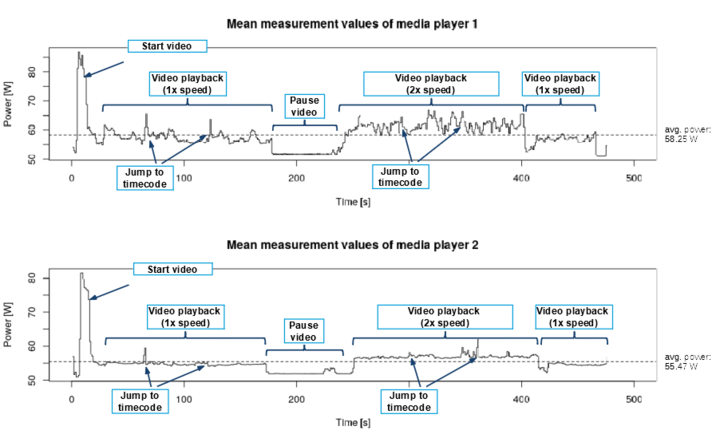
\includegraphics[width=1.1\linewidth]{Mediaplayer.png}
\caption{{\centering 
Vergleich der Leistungsaufnahme von zwei Media-Playern beim Abspielen einer Videodatei. \cite{Guldner22}
}}
\label{mediaplayer}
\end{figure}
Im Anschluss an die Messungen können die gesammelten Daten analysiert und ggf. grafisch dargestellt werden. In \autoref{mediaplayer} ist zu sehen, dass „media player 2“, bei der Ausführung der gleichen Aufgaben im Durchschnitt mit 2,78 W weniger Energie als „media player 1“ verbraucht. Mittels dieser Technik lässt sich also eine simple Beurteilung der Ressourceneffizienz erstellen. \cite{Guldner22}
\newline
\newline
Im Bereich des Cloud Computings gibt es von einigen Cloud-Anbietern bereits Werkzeuge, um den Energieverbrauch und den Einfluss eines Software-Produkts auf die Umwelt ohne großen Versuchsaufbau zu messen. Eines dieser Werkzeuge ist Carbon Footprint von Google (siehe \autoref{carbonfootprint}). Mit Carbon Footprint können Kunden der Google Cloud die Brutto-Kohlenstoffemissionen ihrer Cloudnutzung angezeigt bekommen. Dabei ist Carbon Footprint kostenlos in die Anwendungsoberfläche integriert. Neben den kumulierten Brutto-Kohlenstoffemissionen im Laufe der Zeit können diese auch nach Produkt und nach Region gruppiert überwacht werden. IT-Teams und Entwicklern werden somit Kennzahlen bereitgestellt, die dabei helfen können, den CO2-Fußabdruck ihres Unternehmens zu reduzieren. Auch wenn die Emissionen der digitalen Infrastruktur nur einen Teil des ökologischen Fußabdrucks eines Unternehmens ausmachen, ist eine genaue Bilanzierung der IT-Emissionen notwendig, um die Fortschritte bei der Erreichung der Kohlenstoffreduzierung zu messen, die zur Abwendung der schlimmsten Folgen des Klimawandels erforderlich sind. \cite{Talbott21}
\newline
Neben der Anzeige der Brutto-Kohlenstoffemissionen werden auch konkrete Handlungsempfehlungen gegeben. So erkennt Unattended Project Recommender beispielsweise Projekte, die aufgrund ihres Nutzungsverhaltens aufgegeben werden könnten und zeigt diese dem Anwender an. Google gibt an, dass so im August 2022 insgesamt über 600.000 kg CO2 mit gefundenen sanierungsbedürftigen Projekten verbunden waren. \cite{Talbott21}
\begin{figure}[ht]
\centering
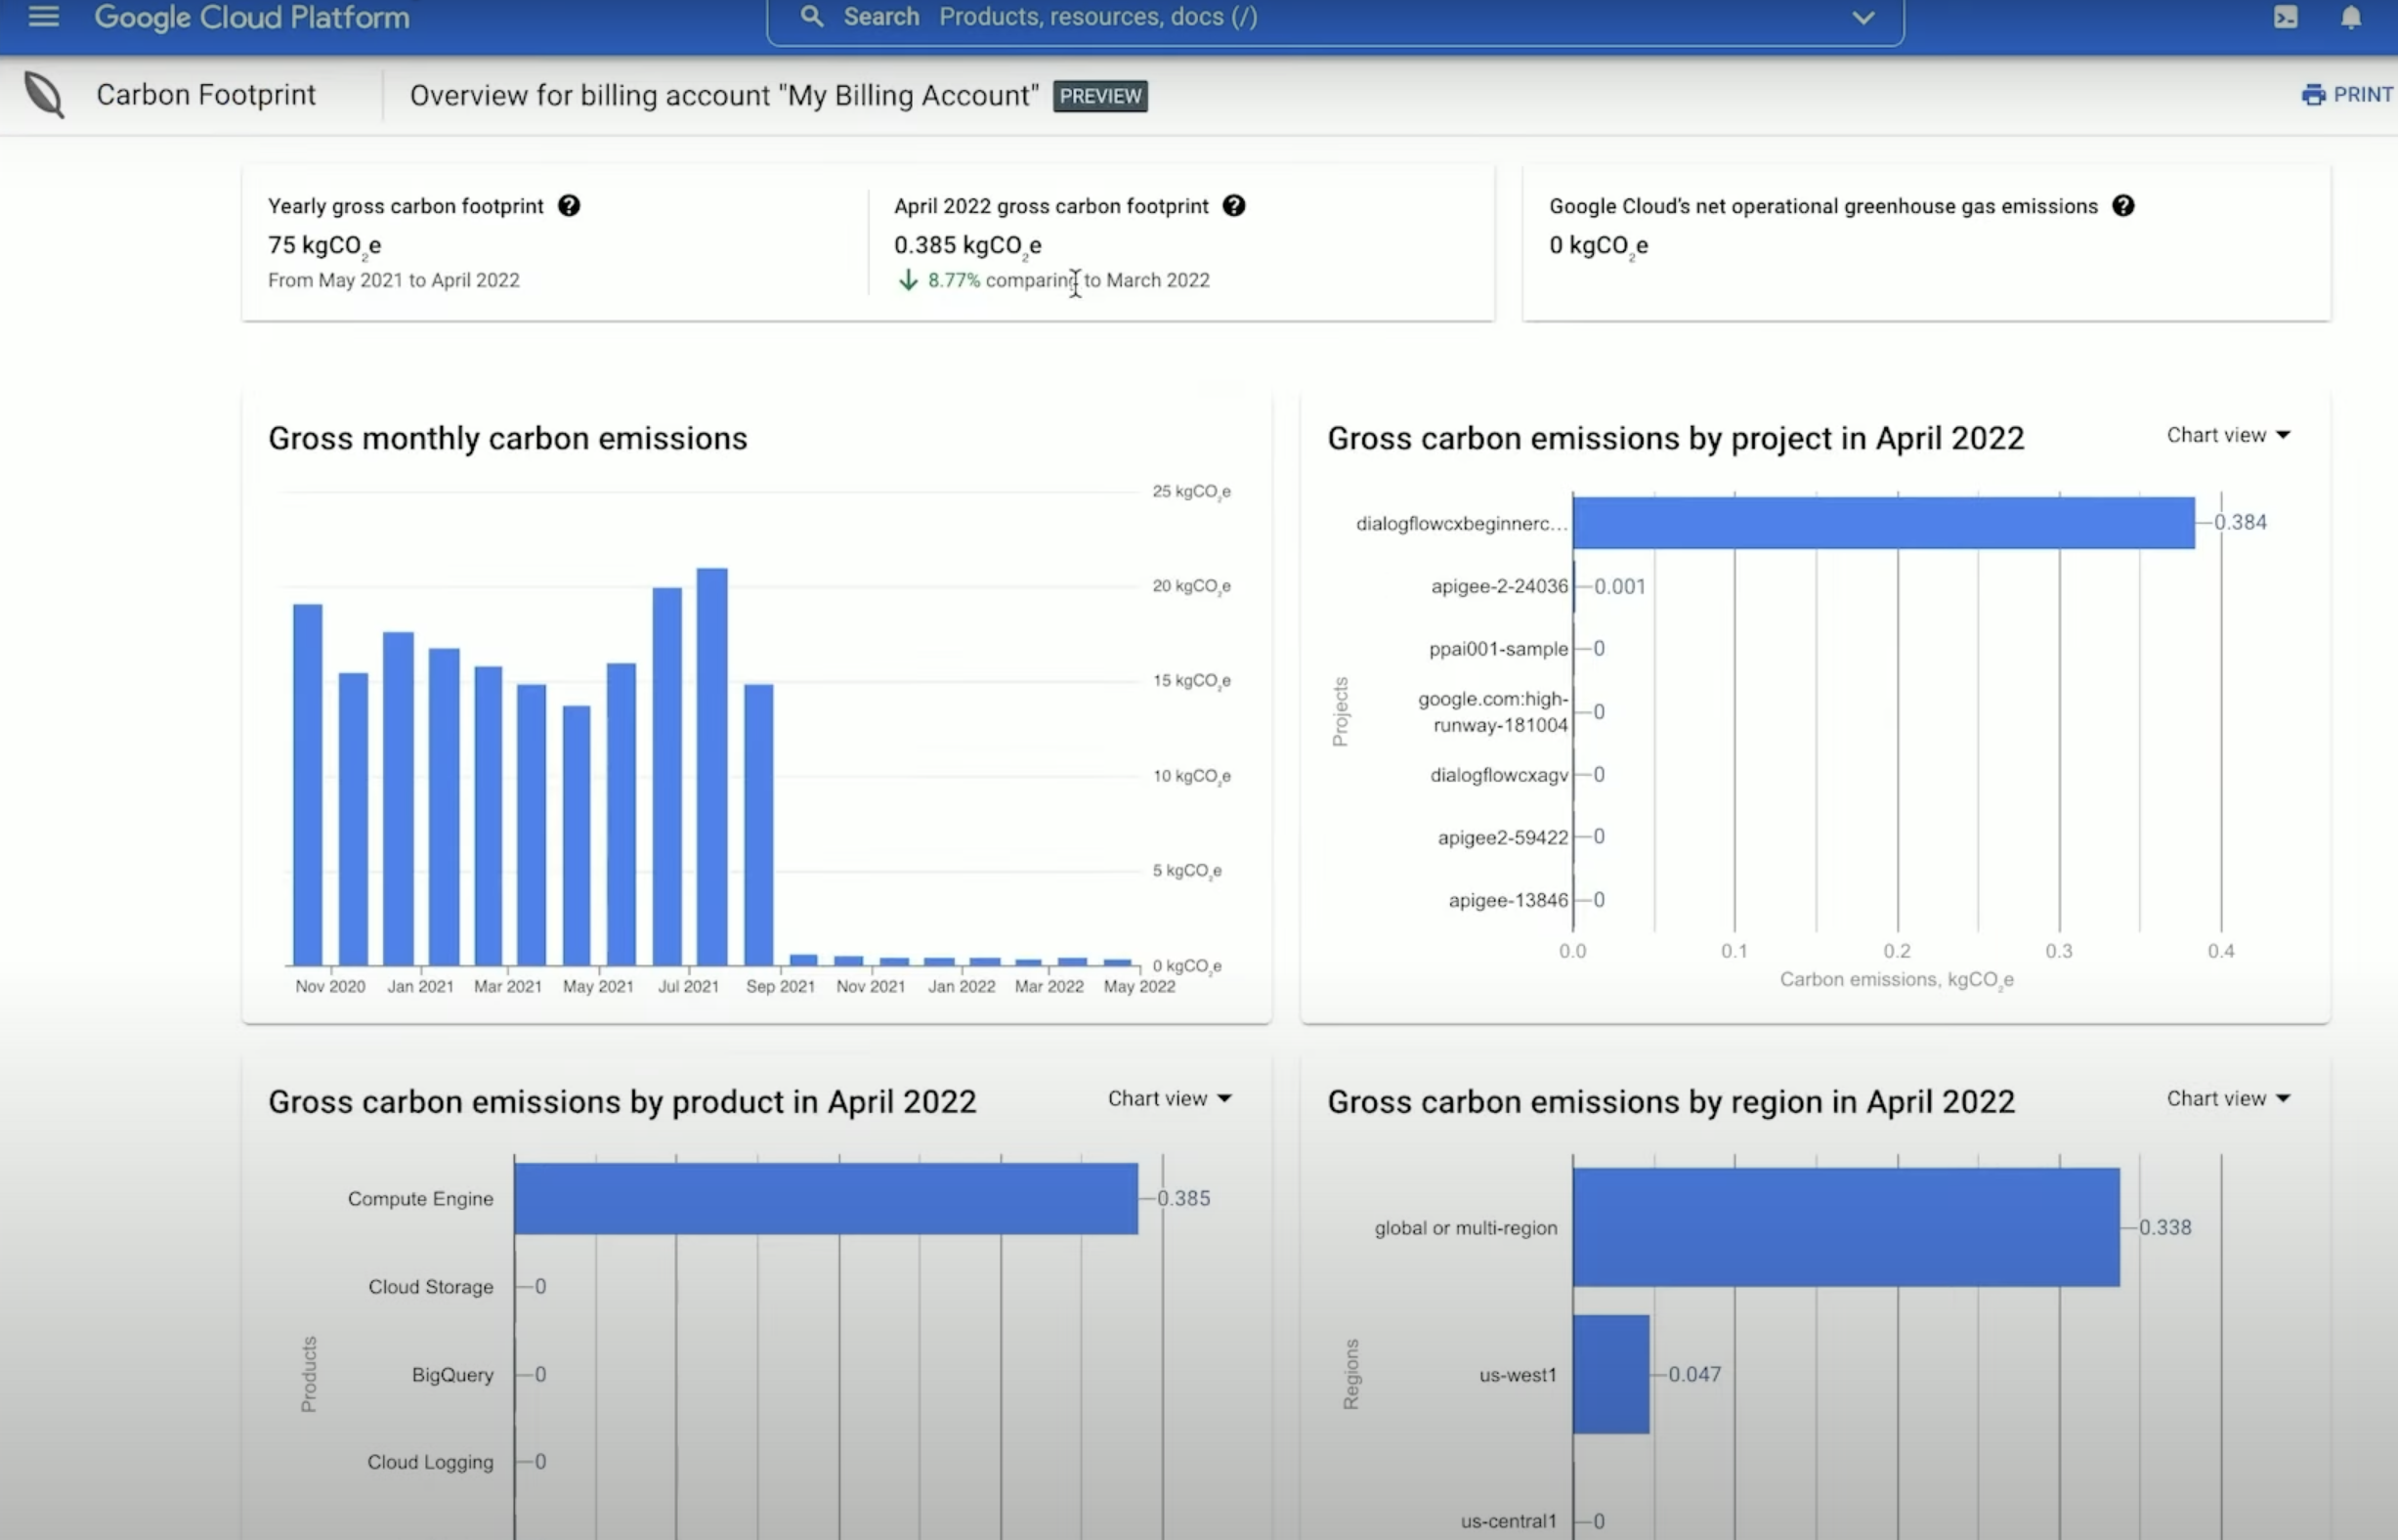
\includegraphics[width=.7\linewidth]{Google-Carbon-Footprint.png}
\caption{{\centering 
Übersichtsseite von Google Carbon Footprint \cite{GoogleCloud.1182022}
}}
\label{carbonfootprint}
\end{figure}

So lässt sich also abschließend aussagen, dass bereits Methoden zur Messung des Verbrauchs von Ressourcen gegeben sind. So kann der Stromverbrauch eines SUT mit dem im Kapitel beschriebenen Versuchsaufbau bestimmt werden. Aber z.B. auch Google bietet mit dem Carbon Footprint schon eine Übersicht über die Brutto-Kohlenstoffemissionen einer bei ihnen gehosteter Cloud-Lösung.

\subsection{Derzeitige Entwicklungen}
\label{Aktuell}
Im Folgenden wird auf die derzeitigen Entwicklungen im IT-Markt eingegangen und inwiefern diese einen Trend hin zur Green IT zeigen oder sogar gänzlich in die andere Richtung. Der wohl größte Trend ist aktuell wohl das wachsende Interesse an der „Cloud“. So bietet Cloud Computing potenziell einen finanziellen Vorteil, da Kunden einen großen, zentral verwalteten Pool von Speicher- und Rechenressourcen gemeinsam nutzen, statt eigene Systeme verwalten zu müssen. \cite{Kondo09} Fraglich ist jedoch, ob diese zentrale Verwaltung auch auf dem Gebiet der natürlichen Ressourcen sparsamer ist. Der Artikel „Green Cloud Computing: Balancing Energy in Processing, Storage, and Transport“ beschäftigt sich mit genau dieser Frage. Die Erkenntnisse aus diesem werden nachfolgend skizziert. Der Begriff Cloud umfasst eine große Menge verschiedener Modelle und Angebote. Der Artikel beleuchtet dabei mehrere Teilgebiete der Cloud, in dieser Arbeit soll jedoch nur auf die zwei Größten davon eingegangen werden: Software as a Service (SaaS) und Storage as a Service (STaaS). SaaS meint das Anbieten einer kompletten Anwendung über die Cloud während STaaS das Outsourcen auf einen Datenspeicher meint. Dabei werden die Daten hochgeladen und müssen für jede Änderung lokal heruntergeladen werden. \cite{Wikipedia22} Wie groß der Energiebedarf der einzelnen Gebiete im Vergleich zur ausschließlichen lokalen Nutzung ist, soll folgend erläutert werden.

\textit{Software as a Service} \newline
\autoref{saas} zeigt ein Diagramm, das den Stromverbrauch (W) pro Nutzer angibt, gemessen an Bildern pro Sekunde (1/s). Ändern sich jede Sekunde 100\% des Bildschirms entspricht dies 1 Bild pro Sekunde. Angegeben sind jeweils private und öffentliche Services mit 20 und 200 Nutzern pro Server. Privat und öffentlich bezieht sich dabei auf die Art des Transport-Netzwerks. Bei Ersterem wird ein firmeninternes Netz verwendet, in Letzterem das öffentliche Internet. Ergänzend wird der Stromverbrauch eines leistungsschwachen und eines durchschnittlichen Laptops im Leerlauf gegenübergestellt.

\begin{figure}[ht]
\centering
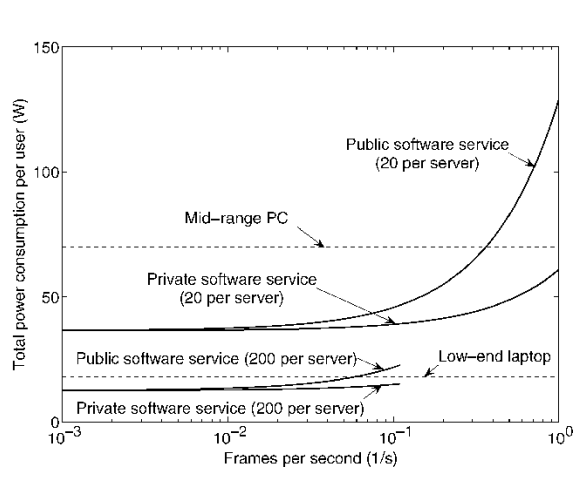
\includegraphics[width=.6\linewidth]{saas.png}
\caption{{\centering 
Stromverbrauch pro Nutzer einer privaten und öffentlichen Cloud je Bild pro Sekunde Rate. \cite{ Baliga11}
}}
\label{saas}
\end{figure}

\autoref{saas} zeigt, dass vor allem bei wenigen Veränderungen der Seite einer Anwendung die Cloud-Lösungen mit 200 Nutzern deutlich stromsparender sind als eigene Rechner, da diese zum Teil im Leerlauf bereits mehr Energie verbrauchen. Bei einer hohen Anzahl an Änderungen der 20 Nutzer steigt der Energiebedarf jedoch signifikant an.

\textit{Storage as a Service} \newline
Einen ähnlichen Verlauf zeigt auch \autoref{staas}. Bei einer geringen Anzahl an Downloads, die bei Änderungen notwendig sind, sind die Cloud Versionen um einiges ressourcenschonender im Vergleich zu einer Laptop-internen HDD. Erst ab ca. 9 Downloads pro Stunde wäre dies nicht mehr der Fall.
\begin{figure}[ht]
\centering
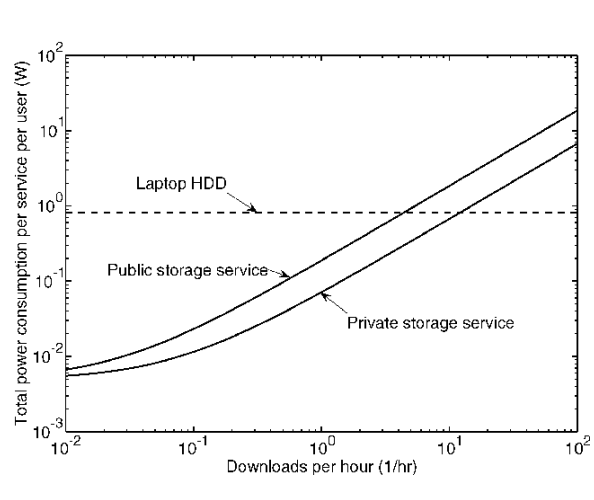
\includegraphics[width=.6\linewidth]{staas.png}
\caption{{\centering 
Pro Nutzer Stromverbrauch je Downloadrate im Vergleich zu einer modernen Laptop HDD. Die durchschnittliche Dokumentengröße beträgt 1,25MB \cite{ Baliga11}
}}
\label{staas}
\end{figure}

Auch für die anderen Teilgebiete wird im Artikel deutlich, dass die Cloud Variante meist stromsparender ist als eine lokale Version. Dies ist vor allem bei geringer Nutzung der Fall und trifft erst für hohe Lasten nicht mehr zu, wie in \autoref{saas} und \autoref{staas} zu sehen ist. \cite{Baliga11}

Die herkömmliche Cloud ist also nicht in den meisten Fällen bereits jetzt ressourcenschonender als der klassische, lokale PC. Zudem gibt es einen wachsenden Bedarf und Forschungsarbeiten hinsichtlich „Green Cloud Computing“, die weitere Potenziale bei der Einsparung von Ressourcen und Strom ausschöpfen wollen. So z.B. auch die Entwicklung von eigens auf die Einsparung von Energie ausgelegten Frameworks. \cite{Chauhan13} Weitere Umsetzungsmöglichkeiten für Green IT sollen im nächsten Kapitel erläutert werden.


\section{Umsetzungsmöglichkeiten}
\label{Umsetzung}
Im Folgenden werden konkrete Umsetzungsmöglichkeiten des Konzepts Green IT beschrieben. Dabei wird zunächst auf Möglichkeiten durch die verwendete Softwarearchitektur eingegangen. Anschließend werden bestimmte Software-Patterns betrachtet und evaluiert, wie durch eine Effizienzsteigerung des Software-Produkts durch diese auch der natürliche Ressourcenverbrauch reduziert werden kann. Abschließend werden Vorgehensmodelle während der Entwicklung eines Software-Produkts betrachtet und deren Einfluss auf den natürlichen Ressourcenverbrauch in der IT-Branche herausgestellt.  

\subsection{Softwarearchitektur}
\label{SWA}
Als erster Teilbereich der Umsetzungsmöglichkeiten soll in diesem Kapitel die Softwarearchitektur beleuchtet werden und mögliche Einsparpotenziale betrachtet werden. In der Literatur gibt es zurzeit noch wenig standardisierte Metriken, die eine Bewertung/Vorhersage der Umweltfreundlichkeit eines bestimmten Softwaresystems, insbesondere während der Entwurfsphase bestimmen könnten. So ist es eine große Herausforderung, insbesondere für Software-Architekten, neue Anwendung möglichst grün zu gestalten. \cite{Mehra22} Auch für bekannte Muster, z. B. Monolithen und Microservices, gibt es noch keine genaueren Studien und Auswirkungen. Unter Beachtung von wenigen allgemeinen Grundsätzen kann auch die Energieeffizienz der Softwarearchitektur verbessert werden.

\textit{Data design, usage and storage} \newline
Um eine gewisse Speicherkapazität bereitzustellen, wird Hardware benötigt, die wiederum Strom verbraucht und zuvor hergestellt werden muss. Ziel sollte also sein, möglichst wenig Daten zu speichern. Auch sollte unnötiger Datenverkehr über das Netzwerk vermieden werden, da dies auch Strom und Ressourcen verbraucht, wie im Kapitel Green IT erklärt.


\textit{Application Design} \newline
Für verschiedene Komponenten sollten Richtlinien definiert werden. So sollte nicht jede Komponente immer aktiv sein, sondern falls sie nicht benötigt wird, abgeschaltet oder zumindest in den Standby-Modus gesetzt werden. Auch ist eine parallele oder asynchrone Verarbeitung sinnvoll. So kann eine nicht zeitkritische Aufgabe während einer Zeit mit möglichst geringer Kohlenstoffintensität berechnet werden.

\textit{Platform deployments, utilization, and scaling} \newline
Ein weiterer wichtiger Punkt ist das Deployment und die Skalierung von Software. So kann bei der Konzipierung der Software auf eine gute Skalierbarkeit der Anwendung geachtet werden. Auch auf den Overhead von Host-Möglichkeiten sollte eingegangen werden. So wird z. B. eine Ausführung der Anwendung abgeschalten, das zugehörige Management-Tool bleibt jedoch aktiv. 

\textit{Code efficiency} \newline
Auch durch den Quelltext selbst gibt es Einsparmöglichkeiten. Code, der aufgrund der Architektur nicht existiert, ist der schnellste Quelltext und somit auch der, der am wenigsten Energie verbraucht. Auch „unnötige“ Arbeit wie z.B. das Erstellen von Log-Dateien, könnte durch verschiedene Service-Level-Agreements für Anwendungen, die dies nicht benötigen deaktiviert werden. Solche nur teilweise benötigten Funktionalitäten können in der Architektur berücksichtigt werden. \cite{Eisele22}

Zusammenfassend gibt es also zwar wenige Vergleiche zwischen konkreten Architekturen, anhand einiger Grundsätze, die auch schon im Kapitel Green IT beschrieben wurden, können jedoch mit bestimmten Design-Entscheidungen Erfolge erzielt werden.


\subsection{Software-Entwurfsmuster}
\label{SWP}
Auch eine Einsparung von Ressourcen durch die Verwendung oder Vermeidung bestimmter Software-Entwurfsmuster ist möglich. Softwareentwickler können durch ein besseres Verständnis der Auswirkungen von Design- und Implementierungsentscheidungen auf Anwendungsebene eine wichtige Rolle bei der Reduzierung des Energieverbrauchs der von ihnen geschriebenen Anwendungen einnehmen. \cite{Sahin12}
\newline
\cite{Sahin12} untersuchte den Energieverbrauch verschiedener Entwurfsmuster. Dabei wurde für dasselbe Programm ohne ein Entwurfsmuster und unter Verwendung eines Entwurfsmusters der jeweilige Energieverbrauch in Joule mittels eines dafür entwickelten Programms gemessen. Die Entwurfsmuster wurden dabei in die drei Kategorien Erstellungsmuster, strukturelle Muster und Verhaltensmuster eingeteilt. Im Folgenden werden die wichtigsten Erkenntnisse daraus dargestellt.
\newline
Erstellungsmuster befassen sich mit der Bereitstellung alternativer Wege zur Erstellung von Objekten. Während die Entwurfsmuster Builder (+1,19\%) und Singleton (+0,42\%) eine Zunahme im Energieverbrauch bewirken, kann mit Factory Method (-0,07\%) eine Reduzierung bewirkt werden. Die höchste Zunahme im Energieverbrauch lässt sich dabei unter Verwendung des Abstract-Factory-Patterns feststellen (+21,55\%). Unter Verwendung des Prototyp-Patterns hat sich der Energieverbrauch der Software um -0,93\% reduziert.
\newline
Strukturelle Muster befassen sich mit der Klassen- und Objektkomposition. Das Entwurfsmuster Kompositum erhöht dabei den Energieverbrauch um +5,14\%. Besonders signifikant ist die Erhöhung des Energieverbrauchs aber unter Verwendung des Decorator-Patterns um +712,89\%. Die Entwurfsmuster Bridge (-0,24\%), Flyweight (-58,08\%) und Proxy (-36,47\%) reduzieren den Gesamtenergieverbrauch der Software. 
Das Decorator-Pattern ist das Entwurfsmuster, welches in dieser Evaluation prozentual am meisten zusätzliche Energie benötigt. Als Erklärung könnte hier dienen, dass unter Verwendung des Decorator-Patterns komplexe Objekte dynamisch und ohne Vererbung erzeugt werden. Die Flexibilität, die das Decorator-Pattern bietet, bringt also gleichzeitig einen höheren Energieverbrauch mit sich, da die Struktur des Objekts nicht bereits zur Kompilierungszeit vollständig festgelegt ist. 
\newline
Verhaltensmuster befassen sich mit der Kommunikation zwischen Objekten. Eine Erhöhung des Energieverbrauchs lässt sich hier nur unter Verwendung des Observer-Patterns um +62,20\% feststellen. Die Entwurfsmuster Command (-1,82\%), Mediator (-9,56\%), Strategy (-0,18\%) und Visitor (-7,49\%) reduzieren jeweils den Energieverbrauch.
\newline
Zusammenfassend kann gesagt werden, dass bei einigen Entwurfsmustern die Auswirkung sehr gering, bei anderen mäßig und bei wenigen signifikant ist. Aber auch die Implementierung von Entwurfsmustern, die nur eine geringe Einsparung mit sich bringen, kann schon lohnend sein. In einer typischen Anwendung kann die Implementierung eines Entwurfsmusters millionen- oder milliardenfach ausgeführt werden. Somit kann auch ein geringer Unterschied je Iterationen einen signifikanten Unterschied im Gesamtenergieverbrauch zur Folge haben.
Die Anwendung dieser Entwurfsmuster kann also den Energieverbrauch eines Software-Produkts sowohl erhöhen als auch verringern. Dabei besteht kein Zusammenhang zur Kategorie des Entwurfsmusters. \cite{Sahin12}
\newline
\newline
Trotzdem sieht man in diesem Test mit traditionellen Software-Entwurfsmustern vor allem einen Anstieg des Energieverbrauchs. \cite{Calero21} rät deshalb für kleine Komponenten davon ab, diese Entwurfsmuster zu verwenden und schlägt stattdessen eigene, auf die Reduktion des Energieverbrauchs angepasste, Software-Entwurfsmuster vor.
\newline \newline \textit{Wakelock} \newline
Ein Wakelock ist ein Mechanismus, der das Ausschalten des Bildschirms oder das Aktivieren des Energiesparmodus eines Geräts unterbindet. Er kommt vor allem bei Smartphones zum Einsatz. Wenn der Wakelock nicht ordnungsgemäß freigegeben wird, wird Energie verbraucht, die eingespart werden könnte. Durch das Hinzufügen einer Freigabeanweisung lässt sich dieses Problem umgehen. \cite{Calero21}
\newline \newline \textit{Recycle} \newline
Recycle beschreibt das Vorgehen, Objekte wie Sammlungen oder Datenbankverbindungen nach ihrer Verwendung wieder zu schließen. Geschieht dies nicht, bleibt z. B. die Verbindung geöffnet und andere Objekte desselben Typs können die gleichen Ressourcen nicht effizient nutzen. \cite{Calero21}
\newline \newline \textit{Übermäßige Methodenaufrufe} \newline
Für jeden Methodenaufruf ist es nötig, dass alle Argumente auf den Stack gelegt, der Rückgabewert im Prozessorregister gespeichert und der Stack aufgeräumt werden muss. Wird eine Methode nun innerhalb einer Schleife mehrfach aufgerufen, wird durch diese Prozedur der Energieverbrauch der Anwendung gesteigert. Als Alternative können z. B. Methodenaufrufe ohne Parameter und auf die durch ein Objekt zugegriffen wird, das innerhalb der Schleife nicht umgewandelt wird, ersetzt werden. Eine Variable, die außerhalb der Schleife deklariert und mit dem Rückgabewert des extrahierten Methodenaufrufs initialisiert wird, kann ohne erneuten Methodenaufruf bei jedem Schleifendurchlauf integriert werden. \cite{Calero21}
\newline \newline \textit{Dynamische Wiederholungsverzögerung} \newline
Wenn von einer Anwendung Daten mit verschiedenen anderen Ressourcen, wie einem Server, ausgetauscht werden, kann es vorkommen, dass die Kommunikation zwischen diesen Ressourcen fehlschlägt. Ist dies der Fall, muss ein erneuter Versuch des Datenaustauschs unternommen werden. Ist die angefragte Ressource jedoch über einen längeren Zeitraum nicht verfügbar, wird die Anwendung wiederholt versuchen, eine Verbindung herzustellen, was zu einem unerwünschten Energieverbrauch führt. Stattdessen kann nach jedem fehlgeschlagenen Verbindungsversuch die Wartezeit vor dem nächsten Versuch linear oder exponentiell erhöht werden. Nach erfolgreicher Verbindung wird die Wartezeit wieder auf den Ursprungswert gesetzt. \cite{Calero21}
\newline \newline \textit{Push over Poll} \newline
Um eine Aktualisierung von Anwendungsdaten zu bewirken, werden von der Anwendung typischerweise Aktualisierungen bei einer anderen Ressource angefragt, zum Beispiel bei einem Server. Dieses kontinuierliche Anfragen von aktualisierten Daten kann jedoch dazu führen, dass einige Anfragen getätigt werden, obwohl keine aktualisierten Daten vorliegen. Als Alternative können Push-Anfragen statt Poll-Anfragen verwendet werden. Das bedeutet, dass die Ressource aktiv Benachrichtigungen an die Anwendung versendet, sobald aktualisierte Daten vorliegen. \cite{Calero21}
\newline \newline \textit{Batch-Operationen} \newline
Die getrennte Ausführung von Operationen führt zu einem überflüssigen Energieverbrauch, der mit dem Ein- und Ausschalten einer bestimmten Ressource zusammenhängt - dies wird typischerweise als "tail energy consumption" bezeichnet. Indem mehrere Vorgänge in einem Einzigen kombiniert werden, wird der Energieverbrauch im Hintergrund optimiert und so Strom eingespart. \cite{Calero21}
\newline \newline \textit{Caching} \newline
In vielen Anwendungen werden Daten von einem entfernten Server abgerufen. Während der Lebensdauer einer solchen Anwendung ist es möglich, dass dieselben Daten mehrmals vom Server abgerufen werden. Um die Netzwerkauslastung zu reduzieren, kann Caching zum Einsatz kommen. Dabei wird das Abrufen von Daten vom Server vermieden, indem diese im Cache vorgehalten werden und verwendet werden können. \cite{Calero21}
\newline
\newline
Unter Verwendung dieser Entwurfsmuster kann der Energieverbrauch eines Software-Produkts reduziert werden. Aber auch Muster, die nicht auf energiebezogene Probleme abzielen, können einen erheblichen Einfluss auf den Energieverbrauch haben. Daher ist es von entscheidender Bedeutung, nicht nur die im System verwendeten Muster zu kennen, sondern auch zu wissen, wie man ihre Vorteile nutzen und gleichzeitig Nachteile für den Gesamtenergieverbrauch des Systems vermeiden kann. \cite{Calero21}

\subsection{Vorgehensmodelle}
Bei der Beantwortung der Fragestellung, wie ein Softwareprodukt nachhaltiger gestaltet werden kann, müssen auch Vorgehensmodelle in der Softwareentwicklung betrachtet werden. Hierbei ist vor allem zu betrachten, wie Entwicklungsprozesse eine Auswirkung auf die Umwelt haben. Der klassische DevOps-Prozess\footnote{DevOps steht für Development and Operations und meint, dass ein Team gemeinschaftlich für die Entwicklung, die Qualitätssicherung und Operationen verantwortlich ist.} fokussiert sich auf Aspekte wie die Reduzierung der Markteinführungszeit oder die Verringerung von menschlichen Fehlern, wohingegen Aspekte der Nachhaltigkeit und Green IT hier aktuell wenig bis keine Beachtung finden. \cite{Brode22} 
\newline
Hierbei ist in erster Linie auf den Stromverbrauch des Software-Produkts zu achten, aber auch Emissionen, die während des Produktionsprozesses der verwendeten Hardware entstanden sind, sollten betrachtet werden.
\newline
Wie aus anderen Bereichen des Software Engineering bekannt ist es deutlich schwieriger und teurer, Änderungen im Anschluss an die Entwicklung oder sogar nach Markteinführung durchzuführen als in frühen Entwicklungsstadien. Deshalb bietet es sich an, Überlegungen zur Nachhaltigkeit so früh wie möglich in den Designprozess der Software zu integrieren. \cite{Dick13}
\newline
Hierfür ist es nötig, den Lebenszyklus von Software-Produkten zu betrachten. Dieser umfasst nach dem \glqq Life Cycle Thinking\grqq{} folgende Phasen: Entwicklung, Vertrieb, Beschaffung, Bereitstellung, Nutzung, Wartung, Deaktivierung und Entsorgung. \cite{Dick10} \newline
In der Entwicklungsphase sind Entwicklungsprozesse zu optimieren. Hier müssen Aspekte wie der tägliche Transportweg zur Arbeit, Dienstreisen oder der Energiekonsum von Arbeitsgeräten betrachtet werden. In den Phasen Vertrieb, Beschaffung und Bereitstellung steht vor allem der Transportweg der Software zum Kunden im Mittelpunkt. Auch bei einem reinen Download kann durch die Downloadgröße Netzwerkverkehr minimiert und so Ressourcen eingespart werden. Bisher betrachtete Möglichkeiten wie \nameref{SWA} (siehe \autoref{SWA}) oder \nameref{SWP} (siehe \autoref{SWP}) können vor allem in der Nutzungsphase Ressourcen einsparen. Hier sind Kriterien wie die Prozessor- und Speicherauslastung, der Netzwerkverkehr, aber auch die Update-Häufigkeit und -Größe zu betrachten. In der Wartungs- und Deaktivierungs-Phase ist die Größe der erstellten Backups ein Kriterium. Auch wie die Daten gespeichert werden, spielt eine Rolle. Die letzte Phase Entsorgung behandelt vor allem, was mit gedruckten Anleitungen, Verpackungen und dem Datenmedium geschieht. \cite{Dick10} \cite{Johann11}
\newline
\newline
Eine Möglichkeit, das bestehende Vorgehensmodell zu optimieren, sind Prozess-Assessments. Hierbei werden Daten gesammelt und sich auf Auswirkungen konzentriert, die sich aus dem Softwareprozess selbst ergeben. Die gesammelten Daten müssen dabei umfangreich genug sein, um eine Kohlenstoff-Fußabdruckberechnung oder eine Lebenszyklusanalyse durchzuführen. Diese Aktivität sollte sehr früh begonnen werden, möglicherweise bereits in der Anfangsphase des Produktdesigns. Dabei wird sich vor allem auf die Entwicklungsphase und mögliche Auswirkungen durch diese konzentriert. Gefundene Schwachstellen können verbessert werden, um so bereits während der Entwicklung Ressourcen einzusparen. \cite{Dick13}
\newline
Indem Administratoren ressourcenschonende Standardkonfigurationen definieren oder die Benutzer zu einem nachhaltigeren Verhalten anleiten, zum Beispiel, indem nach Verlassen des Arbeitsplatzes, dieser in den Ruhezustand versetzt wird, kann während der Entwicklungsphase bereits Energie der Arbeitsgeräte eingespart werden. \cite{Johann11} 
\newline
Zusätzlich können Sustainability Reviews und Previews durchgeführt werden. Diese fokussieren sich auf die Vertriebs-, Beschaffungs-, Bereitstellungs- und Nutzungs-Phase im Vordergrund. Durch verschiedene Werkzeuge und Methoden wie Code-Reviews, Laufzeiteffizienz- und Leistungsmessungen, Energieeffizienzmessungen oder andere Metriken soll hierbei die geleistete Arbeit in Bezug auf Nachhaltigkeitsthemen überprüft werden. Indem Sustainability Reviews und Previews nach etwa zwei Dritteln einer Iteration durchgeführt werden, ist es dem Entwicklungsteam möglich, gefundene Fehler noch innerhalb derselben Iteration zu korrigieren. \cite{Dick13}
\newline
Erkenntnisse aus Sustainability Reviews und Previews, die auch für die Anwender relevant sein könnten, können diesen zur Verfügung gestellt werden. So werden sie in die Lage versetzt, die Auswirkungen auf die Nachhaltigkeit durch ihr Nutzungsverhalten zu optimieren. \cite{Johann11} 
\newline
Auch Retrospektiven zur Nachhaltigkeit sind möglich. Durch diese soll nicht das aktuelle Projekt, sondern die Nachhaltigkeit künftiger Softwareprojekte verbessert werden. Eine solche Retrospektive kann nach Abschluss des Projekts durchgeführt werden, wobei Ergebnisse in Form von gelernten Lektionen, Best Practices, Entscheidungen für zukünftige Projekte etc. dokumentiert werden. \cite{Dick13}
\newline
\newline
Diese Methoden müssen nun in das bestehende Entwicklungsvorgehen integriert werden. In vielen modernen Softwareprojekten wird Scrum als Vorgehensmodell verwendet. Das Ziel von Scrum ist es dabei, in kurzen Iterationen zu arbeiten und in jeder dieser Iterationen ein potenziell auslieferungsfähiges Inkrement der Software zu erstellen. Die bereits in Scrum vorhandenen Bestandteile wie das Sprint Planning, Daily Scrums, Sprint Reviews und die Sprint Retrospective bleiben erhalten und werden durch die beschriebenen Möglichkeiten zur Optimierung der Nachhaltigkeit nicht beeinflusst.
Das Prozess-Assessment ist dabei eine eigene Aufgabe am Anfang des Projekts, um den aktuellen Stand zu evaluieren. Sustainability Reviews und Previews werden in jedem Sprint nach etwa zwei Dritteln von diesen durchgeführt. Die Retrospektive zur Nachhaltigkeit findet einmalig kurz vor dem Ende des Projekts, allerdings noch vor dem letzten Sprint Review statt, um hier das Entwicklungsteam in die Lage zu versetzen, die kombinierten Bewertungsergebnisse an den Product Owner zu berichten. \cite{Dick13}
\newline
\newline
Um diese Vorgehensmodelle umsetzen zu können, muss das Entwicklungsteam durch bestimmte Werkzeuge unterstützt werden. Ein heutzutage viel verwendetes Konzept ist Continuous Integration. Indem die bestehende Continuous Integration Umgebung um eine automatisierte Messung der Energieeffizienz erweitert wird, erhält das Entwicklungsteam zu jedem Zeitpunkt den aktuellen Status hinsichtlich der Energieeffizienz ihres Software-Produkts. So wird es möglich, getätigte Änderungen auch im Hinblick auf Nachhaltigkeit zu bewerten. Dabei ist jedoch zu beachten, dass bereits vorhandene Tests in der Regel ungeeignet für eine Messung der Energieeffizienz sind. Für diese sind Tests nötig, die eine erhebliche Last über einen längeren Zeitraum erzeugen. Das Entwicklungsteam muss dafür optimierte Tests also vorab erstellen. \cite{Dick13}

\section{Gewährleistung, dass Software nachhaltig bleibt}
Durch die in im letzten Kapitel dargestellten Möglichkeiten wurden messbare Werte, wie z.B. der durch Anwendungen verbrauchte Strom idealerweise verringert. Zudem können aufwändigen Berechnungen in ein Rechenzentrum mit besserer Kohlenstoffkonzentration des Stroms verlegt werden.

Als Ziel sollte jedoch auch gelten, dass diese ressourcenschonenden Entwicklungen zukünftig nicht wieder umgekehrt werden. Es sind auch in Zukunft weitere Messungen hinsichtlich des Strombedarfs nötig, um auch nach Erweiterungen einer Anwendung nicht unverhältnismäßig mehr Energie zu verbrauchen. Es muss zudem darauf geachtet werden, dass die programmierte Anwendung auch in Zukunft nutzbar bleibt. Als Faustregel kann dabei auf die Kernfunktionalitäten geachtet werden: Diese sollten auch auf älterer Hardware verfügbar und nutzbar bleiben. \cite{Verdecchia21} Man sollte, wie im \autoref{GreenIT} \nameref{GreenIT} schon genauer beschrieben, nicht durch eine neue Version seine alte Hardware entsorgen müssen, wodurch wieder Kohlenstoff freigesetzt werden würde.

Im \autoref{Umsetzung} \nameref{Umsetzung} wurden Regeln in Bezug auf die Architektur der Software und der Verwendung von bestimmten Entwurfsmuster und Vorgehensmodellen erläutert. Wird sich an diesen orientiert und Muster und Modelle mit Bedacht gewählt, ist dies bereits ein erster Schritt zu einem Softwareprodukt, das auch in Zukunft energiesparend arbeitet.

Auch Label wie der Blaue Engel können die Einstufung einer Applikation als „grün“ gewährleisten, da diese anhand ihrer Vergabekriterien eine umweltfreundliche Software auszeichnen. Werden diese Kriterien nicht mehr erfüllt, ist auch für die Verbraucher ersichtlich, dass die Anwendung nicht länger ausreichend energie- und ressourcensparend ist. \cite{BlauerEngel20}

\section{Bewertung}
In den vorhergehenden Teilen wurden konkrete Umsetzungsmöglichkeiten vorgestellt, die das Software-Produkt nachhaltiger machen sollen. Ob diese Maßnahmen tatsächlich dazu führen, dass Software-Produkte effizienter werden und damit Ressourcen einsparen, lässt sich nicht allgemein belegen. Ohne diese Maßnahmen auszuprobieren und hier Messungen durchzuführen wird diese Frage jedoch weiterhin offen bleiben. \cite{Calero21}
\newline
Auch wurden in dieser Arbeit lediglich Umsetzungsmöglichkeiten auf Software-Seite betrachtet. Eine vollumfängliche Green-IT-Strategie eines Unternehmens muss zwingend auch Überlegungen und Maßnahmen zur Verwendung von Hardware treffen. Im Rahmen dieser Arbeit wird dies mit Fokus auf das Thema gänzlich außen vorgelassen.
\newline
\newline
Generell birgt Green IT sowohl Vorteile als auch Nachteile. Der wohl größte Vorteil ist die Einsparung von Energie. Dies beeinflusst mehrere weitere, nicht zu vernachlässigende Faktoren. Zum einen hat ein geringerer Energieverbrauch der Software-Produkte eines Unternehmens durch Green IT zur Folge, dass die Umweltbelastung (siehe \autoref{GreenIT} \nameref{GreenIT}) durch dieses Unternehmen reduziert wird. 
\newline
Zum anderen sehen sich Unternehmen heutzutage mit deutlich erhöhten Energiekosten konfrontiert. Zusätzlich müssen diese ggf. mit weiteren staatlichen Abgaben rechnen, sofern sie die Umweltauswirkungen ihrer Produkte nicht berücksichtigen. Auch einige Investoren und Verbraucher haben bereits damit begonnen, beim Kauf von Produkten auf die Nachhaltigkeit der Unternehmen zu achten oder die Aktienkurse von Unternehmen abzuwerten, die die von ihnen verursachten Umweltprobleme nur unzureichend angehen. Die Menschen haben begonnen, umweltfreundliche Eigenschaften auch im Bereich der Software zu schätzen. \cite{Murugesan08} Durch den Fokus auf Green IT können also sowohl direkte Kosten in Form von Energie eingespart werden, als auch Verbraucher und Investoren dazu animiert werden, sich für das Unternehmen zu entscheiden.
\newline
Da bereits eine Vielzahl an Green-IT-Kennzahlen und einige Ansätze für Kennzahlsysteme vorhanden sind, wird die Bestimmung von Ansatzpunkten für Green IT vereinfacht.
\newline
\newline
Auf der anderen Seite ist jedoch eine hohe Fachkompetenz erforderlich, um die Kennzahlen zu analysieren und geeignete Maßnahmen für Green IT abzuleiten. Aus wirtschaftlicher Sicht ist es deshalb nicht sicher, ob die Integration von Green-IT-Maßnahmen sinnvoll ist, da durch die Bestimmung und Integration geeigneter Maßnahmen ggf. höhere Kosten entstehen könnten, als sie durch den Nutzen dieser Maßnahmen eingespart werden. 
\newline
Da in einem gewinnorientierten Unternehmen hauptsächlich monetäre Aspekte im Vordergrund stehen, wird der Nutzen von Green-IT-Maßnahmen oft übersehen und sich dagegen entschieden. Dabei spielen sowohl die Kosten der Integration von Maßnahmen, aber auch ggf. auftretende Leistungs-Einbußen der Software sowie Wartungskosten eine Rolle.
\newline
Auch Greenwashing ist ein potenzieller Nachteil von Green IT. Einige Unternehmen haben das Potenzial erkannt, durch vermeintliche Umweltschutzkampagnen einen höheren Kundenkreis für sich gewinnen oder Investoren zu einer Investition überzeugen zu können. Greenwashing meint dabei den Versuch von Unternehmen durch Kommunikation, Marketing und Einzelmaßnahmen ein \glqq grünes Image\grqq{} zu erlangen, ohne entsprechende Maßnahmen im operativen Geschäft systematisch verankert zu haben. \cite{LinHi21} 
\newline
\newline
Insgesamt ist Green IT jedoch ein guter und mit Blick auf den menschengemachten Klimawandel wichtiges Konzept, das jedes Unternehmen zeitnah integrieren sollte. Dabei kann auch die Seite der Software geprüft und entsprechende Maßnahmen für diese abgeleitet werden.

\section{Ausblick}
Mittels der Anwendung von Konzepten der Green IT kann ein Unternehmen nicht nur mehr zum Umweltschutz generell beitragen, sondern auch durch den Betrieb von Software entstehende Kosten reduzieren. Neben hardwareseitigen Umsetzungsmöglichkeiten kann durch die Verwendung bestimmter Entwurfsmuster, die Wahl einer ressourcensparenden Architektur und des Etablieren bestimmter Vorgehensmodelle auch seitens der Software selbst dazu beigetragen werden, dass diese nachhaltiger wird. 
\newline
Unter Beachtung der Vorteile von Green IT ist zu erwarten, dass zukünftig noch deutlich mehr Unternehmen dieses Thema fokussieren werden. Jedes Unternehmen muss eine ganzheitliche, umfassende Green-IT-Strategie entwickeln. Anschließend sollte es eine Green-IT-Politik entwickeln, die Ziele, Aktions- und Zeitpläne enthält. Große Unternehmen sollten auch einen Beauftragten für ökologische Nachhaltigkeit ernennen, der ihre grüne Strategie umsetzt und ihre Fortschritte und Erfolge überwacht. \cite{Murugesan08}
\newline
Auch die Forschung wird sich durch die große Bedeutung in der Industrie künftig verstärkt mit Green IT und zugehörigen Maßnahmen auseinandersetzen. 
\newline

%% \bibliography{lni-paper-example-de.tex} ist hier nicht erlaubt: biblatex erwartet dies bei der Preambel
%% Starten Sie "biber paper", um eine Biliographie zu erzeugen.
\printbibliography

\end{document}
